\section{Kết quả thí nghiệm}
\subsection{Pha khám phá}
Sau khi hoàn tất quá trình khám phá, đồ án tiến hành đánh giá hiệu suất của phương pháp ước lượng trọng tâm bằng cách so sánh khoảng cách từ điểm trọng tâm ước lượng đến điểm trọng tâm thật trên 3 vật thể được chọn với các cấu hình đánh giá khác nhau. Mỗi cấu hình đánh giá bao gồm số lượng cạnh xét ngẫu nhiên (tối thiểu là 2), số mẫu trên mỗi cạnh (tối thiểu là 3) và lực đẩy tối đa $f_\text{max0}$ trong pha khám phá, thực hiẹn 1000 lần chạy thử nghiệm. Để đảm bảo tính công bằng giữa các lần thí nghiệm, tất cả các lần chạy đều sẽ sử dụng chung bộ sinh số ngẫu nhiên, nhiều gauss được thêm vào thành phần đo gia tốc. Ngoài ra để sinh cánh tay đòn lớn và đều hơn thì vị trí mẫu sẽ không được sinh ngẫu nhiên mà chia đều theo hai đầu mút của cạnh trong không gian làm việc. Kết quả thí nghiệm có thể được minh họa trong hình \ref{fig:box_plot}:
\begin{figure}[!h]
    \centering
    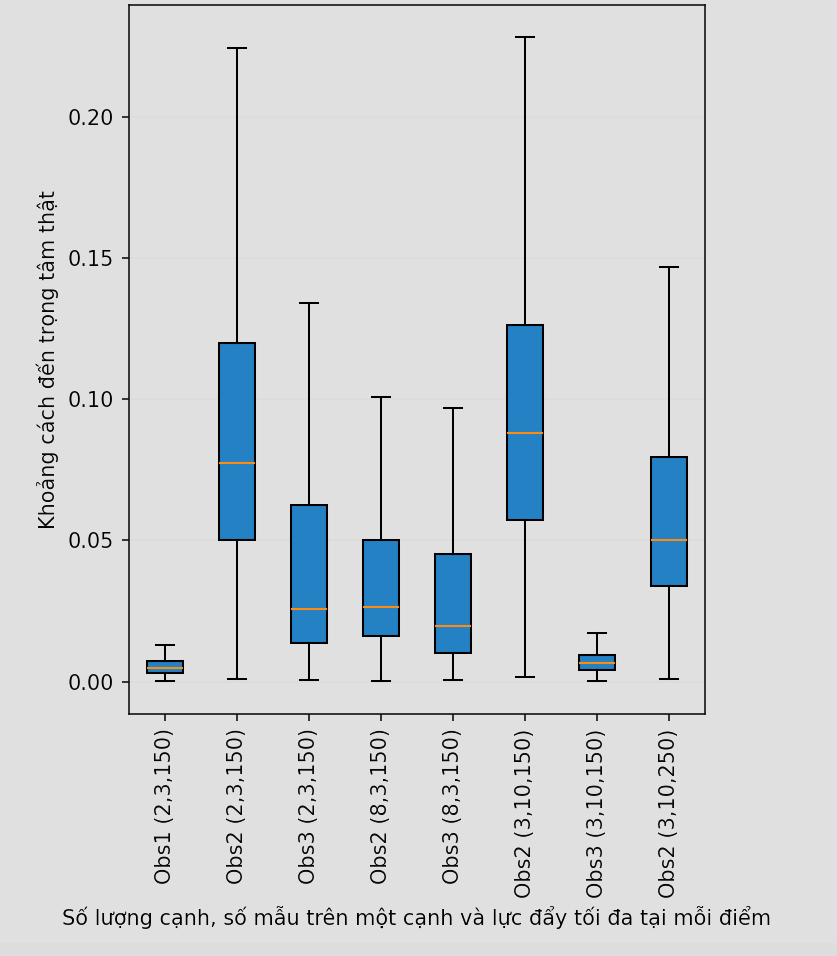
\includegraphics[width=0.5\textwidth]{chapter2/image/box_plot.png}
    \caption{Kết quả thí nghiệm ước lượng trọng tâm} 
    \label{fig:box_plot}
\end{figure}

trong đó các vật thể hình chữ nhật, chữ T và ngôi sao lần lượt được ký hiệu là Obs1, Obs2 và Obs3.

Đầu tiên, rất dễ nhận ra vật thể hình chữ nhật cho ra sai số tốt nhất, gần như sát điểm trọng tâm với cấu hình mặc đỉnh là 2 cạnh và 3 lần đẩy thử trên mỗi cạnh. Điều này là do vật là một đa giác lồi, hình chiếu của trọng tâm luôn nằm trên cạnh của vật, ngoài ra cánh tay đòn trên mỗi cạnh đều có thể cho ra một gia tốc đủ lớn. Hai vật còn lại cho kết quả kém hơn, đặc biệt là vật hình chữ T khi trung vị gần 7cm. Lý do là do hai vật này sở hữu các cạnh mà hình chiếu của trọng tâm nằm ngoài cạnh đó, đồng thời các cạnh ở chân và hai bên đầu chữ T quá ngắn, làm cho gia tốc góc chịu ảnh hưởng nhiều hơn do nhiễu. Khi gia tốc góc quá bé, sau khi cộng thêm với nhiễu sẽ làm giá trị của nó lệch đi rất nhiều so với ban đầu, dẫn đến lúc tính trọng tâm ta giải ra các điểm ở rất xa so với tâm thật. Ta có thể lọc các trường hợp này khi thấy khoảng cách sai số lớn hơn 1m, do bán kính đường tròn bé nhất tâm là điểm trọng tâm mà vật nằm trong cũng xấp sỉ giá trị này. Trong số 1000 lần chạy thử, xác suất xuất hiện các trường hợp này là khoảng $2\%$.

Khi tăng số lượng cạnh mỗi lần chạy lên, có thể thấy độ chính các của vật hình chữ T cải thiện hơn, do kết quả được tổng hợp từ đầy đủ các cạnh, trong đó các cạnh tốt sẽ làm giảm sai số trung bình đi đáng kể, vào khoảng 3cm. Đối với hình ngôi sao kết quả không thay đổi đáng kể do mỗi cạnh của nó đều như nhau. Do đó để kết quả ổn định, đồ án đề xuất nên xét hết tất cả các cạnh của vật thể thay vì chỉ 2 cạnh.

Đối với việc tăng số mẫu trên một cạnh, với cấu trúc vật đều như của hình ngôi sao thì kết quả rất tốt, tiệm cận với trọng tâm thật khi phép hồi quy hoạt động hiệu quả, tuy nhiên nếu đã có những cạnh quá ngắn như hình chữ T thì kết quả gần như không cải thiện gì. Trong khi đó việc tăng lực đẩy tối đa mỗi lần đẩy sẽ luôn cho kết quả tốt hơn do gia tốc góc tạo được đủ lớn để không bị ảnh hưởng bởi nhiễu. Điều này làm củng cố thêm ý nghĩa của khả năng mở rộng đã nói ở trên của phương pháp này, khi ta nên dùng nhiều robot cùng khám phá để có kết quả chính xác hơn.

Sau khi lựa chọn tham số hợp lý, kết quả cho thấy sai số trung bình sẽ vào khoảng 3-7cm tùy theo $f_\text{max}$. Đây là một khoảng sai số khá bé khi các cạnh của vật thường dài từ 1-2m. Sai số đủ bé để coi không quá ảnh hưởng đến ma trận Grasp-map, các sai lệch về góc có thể được xem là nhiễu hệ thống để xử lý và sẽ được thực hiện ở mục sau, tuy nhiên sai số có thể khác biệt tùy vào mô hình nhiễu cảm biến trong thực tế. Để kết luận, đồ án đề xuất nên xét tất cả các cạnh của vật thể, hoặc chọn những cạnh tốt có thể sinh được gia tốc góc với chênh lệch đáng kể, ngoài ra cũng có thể tăng số mẫu trên các cạnh này và sử dụng nhiều robot tham gia đẩy để có các kết quả tốt hơn.

\subsection{Pha đẩy vật}

Sau khi ước lượng được một điểm trọng tâm, bầy robot sẽ tiến hành xây dựng đội hình và chiến thuật với cánh tay đòn được tính từ điểm trọng tâm này. Đầu tiên để thử nghiệm khả năng xây dựng đội hình dựa trên wrench mong muốn, 3 wrench mong muốn được chọn đặc trưng cho các chuyển động tịnh tiến thuần, xoay thuần và kết hợp vừa tịnh tiến vừa xoay lần lượt là $[0,40,0]$, $[0,0,60]$ và $[0,-40,-60]$. Mỗi wrench sẽ được thử trên cả 3 vật thể, tổng cộng 9 lần chạy thử nghiệm. Các cấu hình thu được như hình sau:
\begin{figure}[!h]
    \centering
    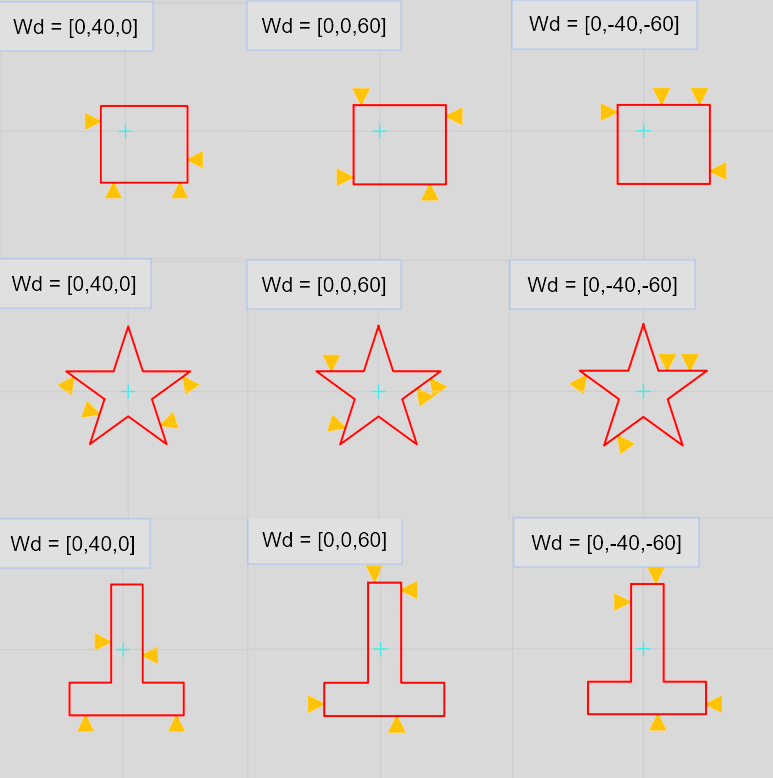
\includegraphics[width=0.5\textwidth]{chapter2/image/form.png}
    \caption{Kết quả thí nghiệm xây dựng cấu hình} 
    \label{fig:form}
\end{figure}

 Do bản chất thuật toán là heuristic, và thật sự tồn tại nhiều hơn một lời giải cho nghiệm tối ưu được chọn, các cấu hình giải ra tại hai lần giải khác nhau có thể khác biệt hoàn toàn dù cùng đầu vào. Tuy nhiên các cấu hình được chọn luôn đảm bảo wrench mong muốn $w_d$ luôn nằm trong không gian làm việc $\mathcal(G)$, do đó nghiệm duy nhất $f_r$ luôn có thể thu được thông qua lời giải của bài toán quy hoạch toàn phương. Với solver OSQP được sử dụng, các nghiệm thu được thường cho ra tổng hợp lực mô men $w_e$ bám rất sát với $w_d$, vật di chuyển nhanh dần đều về hướng wrench mong muốn, sai số chủ yếu là sai số lượng tử và không đáng kể. Kết quả thể hiện rõ tính linh hoạt của thuật toán khi có thể xây dựng được một cấu hình bền vững, có khả năng sinh ra lực-mô men theo mong muốn bất kể đặc tính về hình dạng của vật. 

\begin{figure}[!h]
    \centering
    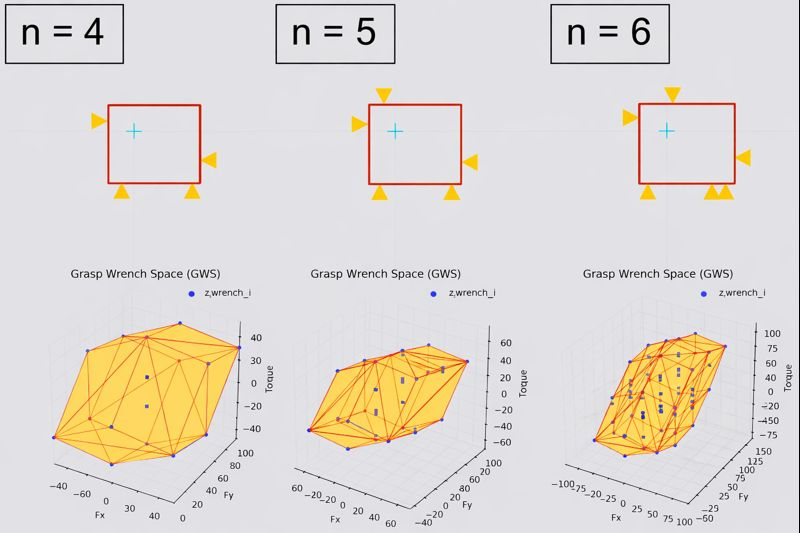
\includegraphics[width=0.7\textwidth]{chapter2/image/image.png}
    \caption{Thay đổi số lượng robot tham gia} 
    \label{fig:change_n}
\end{figure}

Ngoài ra, tính mở rộng của thuật toán còn thể hiện ở việc số lượng cá thể robot tham gia làm việc có thể tăng hoặc giảm theo mong muốn miễn là có tối thiếu số robot cần thiết để sinh ra đủ lực-mô men lên vật sao cho thắng được lực ma sát tĩnh của vật. Qua quá trình thí nghiệm, số robot tối thiểu cần để bắt đầu xây dựng một cấu hình khả thi là 3 robot, do các cấu hình với 2 robot trở xuống thường có không gian làm việc gần như là một mặt phẳng trong không gian wrench space, ngoài ra các cấu hình với 4 robot trở lên thường ổn định hơn, lý thuyết này được chứng minh trong \cite{nguyen1986stable} là cần tối thiểu 4 contact point để đạt được form-closure. Hình \ref{fig:change_n} minh họa các cấu hình thu được khi thay đổi số lượng robot tham gia từ 3 đến 6 robot trên vật hình chữ nhật với wrench mong muốn là $[0,40,0]$. Kết quả cho thấy với số lượng robot càng nhiều, vùng không gian làm việc $\mathcal{G}$ sinh ra càng lớn, đặc biệt là theo trục mô men, dẫn đến cấu hình thu được càng ổn định và đa dạng hơn, đồng thời lực tác dụng lên mỗi robot cũng giảm đi đáng kể, giúp giảm thiểu nguy cơ trượt trong quá trình đẩy vật.

Đồ án cũng có thử đẩy vật theo quỹ đạo đã mong muốn sử dụng mô hình động lực học, tuy nhiên do thuật toán trên được thiết kế cho mô hình bán tĩnh, khi mà tác dụng 1 cố định vào thì vật sẽ chuyển động đều theo một vận tốc cố định, nên khi chuyển sang dynamic sẽ có nhiều yếu tố khó khăn hơn, như không chỉ yêu cầu sai lệch về vị trí mà còn cả sai lệch về vận tốc để tính toán ra lực-mô men mong muốn. Dù chưa có được kết quả hoàn chỉnh, đồ án đã thử nghiệm được một trường hợp khi vận chuyển vật hình ngôi sao theo quỹ đạo mong muốn bằng một bộ điều khiển PD. Số đội hình robot

\begin{figure}[!h]
    \centering
    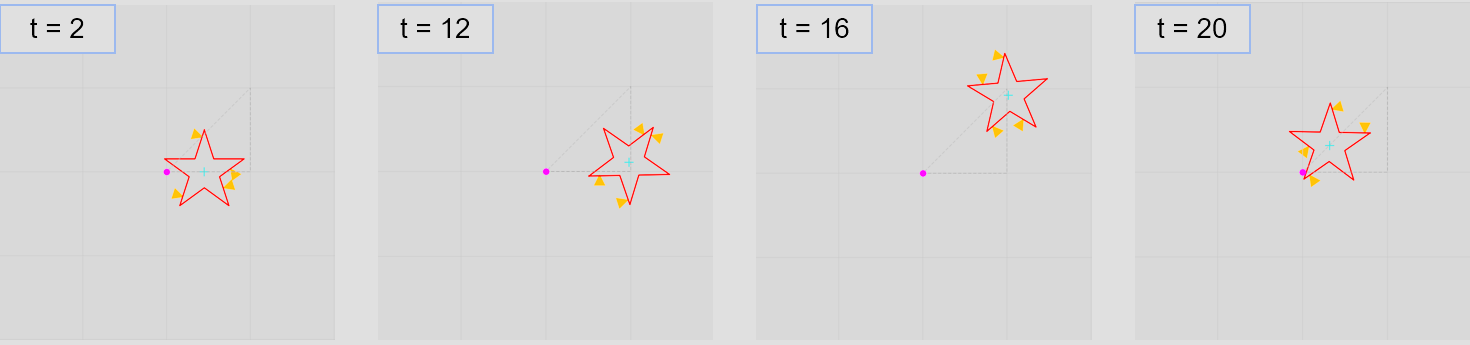
\includegraphics[width=1\textwidth]{chapter2/image/xam.png}
    \caption{Điều khiển vật theo quỹ đạo} 
    \label{fig:xam}
\end{figure}

\begin{figure}[!h]
    \centering
    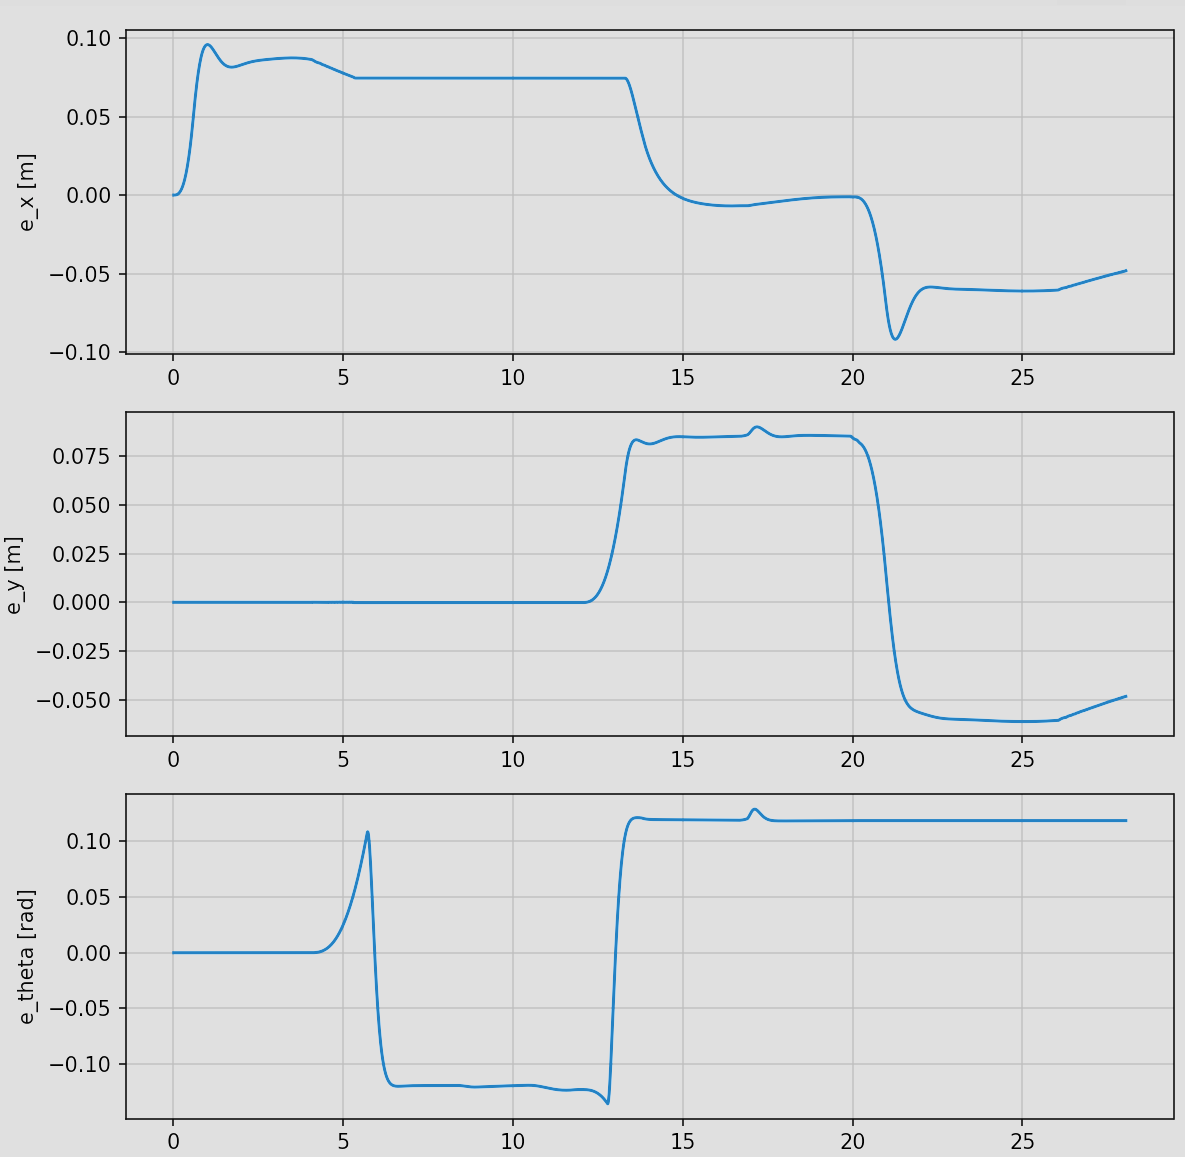
\includegraphics[width=0.7\textwidth]{chapter2/image/saiso.png}
    \caption{Sai sô điều khiển} 
    \label{fig:sai}
\end{figure}

Số lần robot phải đổi cấu hình là 8, trong đó có những lần đổi không cần thiết do $w_d$ tính toán được vượt quá xa so với wrench space. Từ bảng sai số, có thể thấy quá trình đẩy thử nghiệm tương đối ổn định và ít sai số trên những quỹ đạo đẩy thẳng, không cần xoay. Ngược lại, do sai số từ ước lượng COM được coi là nhiễu nên hệ thống còn chưa xử lý tốt chuyển động quay. Ngoài ra do điều khiển theo dynamic nên trường hợp gia tốc tích lũy dẫn đến vận tốc tăng liên tục làm vật bị vọt ló còn cần được xử lý thêm.

